\documentclass{article}
\usepackage{pgf,tikz}
\usetikzlibrary{calc,math}
\begin{document}

%\begin{tikzpicture}[scale=1.2]
%
%%\draw[help lines,very thin](0,0) grid (6,6);
%\tikzmath{
%\h=cos(pi/3);
%\v=sin(pi/3);
%\ah=1.5*cos(45);
%\av=1.5*sin(45);
%\d =cos(30);
%\e =sin(30);
%}
%\coordinate[label=below:\footnotesize$B$] (B) at(0,0);
%\coordinate[label=below:\footnotesize$C$] (C) at(3,0);
%\coordinate[label=right:\footnotesize$D$](D) at($(C)+(\d,\e)$);
%\coordinate[label=left:\footnotesize$A$](A) at($(B)+(\d,\e)$);
%\coordinate[label=above left:\footnotesize$N$](N) at($(D)!0.5!(A)$);
%\coordinate[label=above:$S$](S) at($(N)+(0,2.4)$);
%\draw (B)--(C)--(D);
%\draw[dashed] (B)--(A)--(D) ;
%\foreach \p in{B,C,D}
%\draw (S)--(\p);
%\foreach \p in{A,N}
%\draw[dashed] (S)--(\p);
%\draw [dashed] (C)--(N);
%\end{tikzpicture}
%\begin{tikzpicture}
%\tikzmath{
%\a =cos(45);
%}
%%\draw [help lines](0,0) grid (4,4);
%\coordinate[label=below:$A$](A) at(0,0);
%\coordinate[label=below:$C$](C) at(4,0);
%\coordinate[label=a:$P$](P) at(0,4);
%\coordinate[label=below:$B$](B) at($(4-\a,-\a )$);
%\coordinate[label=right:$H$](H) at($(P)!0.5!(C)$);
%\coordinate[label=below:$M$](M) at($(A)!0.5!(H)$);
%\draw (A)--(B)--(P)--(C)--(B) (P)--(A) (B)--(H);
%\draw[dashed](A)--(H) (A)--(C) (P)--(M);
%\end{tikzpicture}
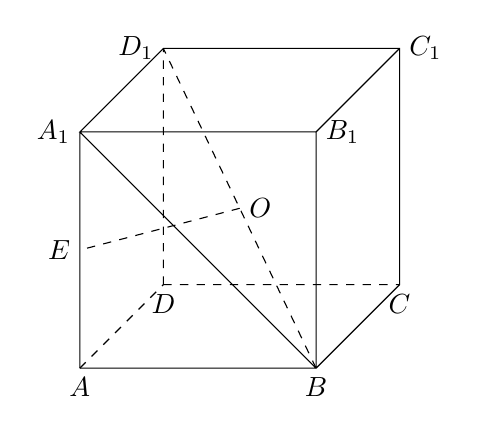
\begin{tikzpicture}
\tikzmath{
\a=cos(45);
\b =1.5*\a;
}
%\draw[help lines] (0,0) grid (3,3);
\coordinate[label=below:$A$](A) at(0,0);
\coordinate[label=below:$B$](B) at(3,0);
\coordinate[label=below:$D$](D) at($(\b,\b)$);
\coordinate[label=below:$C$](C) at($(B)+(D)$);
\foreach \p in{B,C}
\coordinate[label=right:$\p_1$] (\p_1) at($(\p)+(0,3)$);
\foreach \p in{A,D}
\coordinate[label=left:$\p_1$] (\p_1) at($(\p)+(0,3)$);
\coordinate[label=right:$O$](O) at($(B)!0.5!(D_1)$);
\coordinate[label=left:$E$](E) at($(A)!0.5!(A_1)$);
\draw(A)--(B)--(C)--(C_1)--(D_1)--(A_1)--(B_1)--(C_1) (A)--(A_1) (B)--(B_1) (A_1)--(B);
\draw[dashed](A)--(D) (D)--(C) (D)--(D_1) (B)--(D_1) (O)--(E);
\end{tikzpicture}
\end{document}